% Options for packages loaded elsewhere
\PassOptionsToPackage{unicode}{hyperref}
\PassOptionsToPackage{hyphens}{url}
%
\documentclass[
]{article}
\usepackage{amsmath,amssymb}
\usepackage{lmodern}
\usepackage{iftex}
\ifPDFTeX
  \usepackage[T1]{fontenc}
  \usepackage[utf8]{inputenc}
  \usepackage{textcomp} % provide euro and other symbols
\else % if luatex or xetex
  \usepackage{unicode-math}
  \defaultfontfeatures{Scale=MatchLowercase}
  \defaultfontfeatures[\rmfamily]{Ligatures=TeX,Scale=1}
\fi
% Use upquote if available, for straight quotes in verbatim environments
\IfFileExists{upquote.sty}{\usepackage{upquote}}{}
\IfFileExists{microtype.sty}{% use microtype if available
  \usepackage[]{microtype}
  \UseMicrotypeSet[protrusion]{basicmath} % disable protrusion for tt fonts
}{}
\makeatletter
\@ifundefined{KOMAClassName}{% if non-KOMA class
  \IfFileExists{parskip.sty}{%
    \usepackage{parskip}
  }{% else
    \setlength{\parindent}{0pt}
    \setlength{\parskip}{6pt plus 2pt minus 1pt}}
}{% if KOMA class
  \KOMAoptions{parskip=half}}
\makeatother
\usepackage{xcolor}
\usepackage[margin=1in]{geometry}
\usepackage{color}
\usepackage{fancyvrb}
\newcommand{\VerbBar}{|}
\newcommand{\VERB}{\Verb[commandchars=\\\{\}]}
\DefineVerbatimEnvironment{Highlighting}{Verbatim}{commandchars=\\\{\}}
% Add ',fontsize=\small' for more characters per line
\usepackage{framed}
\definecolor{shadecolor}{RGB}{248,248,248}
\newenvironment{Shaded}{\begin{snugshade}}{\end{snugshade}}
\newcommand{\AlertTok}[1]{\textcolor[rgb]{0.94,0.16,0.16}{#1}}
\newcommand{\AnnotationTok}[1]{\textcolor[rgb]{0.56,0.35,0.01}{\textbf{\textit{#1}}}}
\newcommand{\AttributeTok}[1]{\textcolor[rgb]{0.77,0.63,0.00}{#1}}
\newcommand{\BaseNTok}[1]{\textcolor[rgb]{0.00,0.00,0.81}{#1}}
\newcommand{\BuiltInTok}[1]{#1}
\newcommand{\CharTok}[1]{\textcolor[rgb]{0.31,0.60,0.02}{#1}}
\newcommand{\CommentTok}[1]{\textcolor[rgb]{0.56,0.35,0.01}{\textit{#1}}}
\newcommand{\CommentVarTok}[1]{\textcolor[rgb]{0.56,0.35,0.01}{\textbf{\textit{#1}}}}
\newcommand{\ConstantTok}[1]{\textcolor[rgb]{0.00,0.00,0.00}{#1}}
\newcommand{\ControlFlowTok}[1]{\textcolor[rgb]{0.13,0.29,0.53}{\textbf{#1}}}
\newcommand{\DataTypeTok}[1]{\textcolor[rgb]{0.13,0.29,0.53}{#1}}
\newcommand{\DecValTok}[1]{\textcolor[rgb]{0.00,0.00,0.81}{#1}}
\newcommand{\DocumentationTok}[1]{\textcolor[rgb]{0.56,0.35,0.01}{\textbf{\textit{#1}}}}
\newcommand{\ErrorTok}[1]{\textcolor[rgb]{0.64,0.00,0.00}{\textbf{#1}}}
\newcommand{\ExtensionTok}[1]{#1}
\newcommand{\FloatTok}[1]{\textcolor[rgb]{0.00,0.00,0.81}{#1}}
\newcommand{\FunctionTok}[1]{\textcolor[rgb]{0.00,0.00,0.00}{#1}}
\newcommand{\ImportTok}[1]{#1}
\newcommand{\InformationTok}[1]{\textcolor[rgb]{0.56,0.35,0.01}{\textbf{\textit{#1}}}}
\newcommand{\KeywordTok}[1]{\textcolor[rgb]{0.13,0.29,0.53}{\textbf{#1}}}
\newcommand{\NormalTok}[1]{#1}
\newcommand{\OperatorTok}[1]{\textcolor[rgb]{0.81,0.36,0.00}{\textbf{#1}}}
\newcommand{\OtherTok}[1]{\textcolor[rgb]{0.56,0.35,0.01}{#1}}
\newcommand{\PreprocessorTok}[1]{\textcolor[rgb]{0.56,0.35,0.01}{\textit{#1}}}
\newcommand{\RegionMarkerTok}[1]{#1}
\newcommand{\SpecialCharTok}[1]{\textcolor[rgb]{0.00,0.00,0.00}{#1}}
\newcommand{\SpecialStringTok}[1]{\textcolor[rgb]{0.31,0.60,0.02}{#1}}
\newcommand{\StringTok}[1]{\textcolor[rgb]{0.31,0.60,0.02}{#1}}
\newcommand{\VariableTok}[1]{\textcolor[rgb]{0.00,0.00,0.00}{#1}}
\newcommand{\VerbatimStringTok}[1]{\textcolor[rgb]{0.31,0.60,0.02}{#1}}
\newcommand{\WarningTok}[1]{\textcolor[rgb]{0.56,0.35,0.01}{\textbf{\textit{#1}}}}
\usepackage{graphicx}
\makeatletter
\def\maxwidth{\ifdim\Gin@nat@width>\linewidth\linewidth\else\Gin@nat@width\fi}
\def\maxheight{\ifdim\Gin@nat@height>\textheight\textheight\else\Gin@nat@height\fi}
\makeatother
% Scale images if necessary, so that they will not overflow the page
% margins by default, and it is still possible to overwrite the defaults
% using explicit options in \includegraphics[width, height, ...]{}
\setkeys{Gin}{width=\maxwidth,height=\maxheight,keepaspectratio}
% Set default figure placement to htbp
\makeatletter
\def\fps@figure{htbp}
\makeatother
\setlength{\emergencystretch}{3em} % prevent overfull lines
\providecommand{\tightlist}{%
  \setlength{\itemsep}{0pt}\setlength{\parskip}{0pt}}
\setcounter{secnumdepth}{-\maxdimen} % remove section numbering
\ifLuaTeX
  \usepackage{selnolig}  % disable illegal ligatures
\fi
\IfFileExists{bookmark.sty}{\usepackage{bookmark}}{\usepackage{hyperref}}
\IfFileExists{xurl.sty}{\usepackage{xurl}}{} % add URL line breaks if available
\urlstyle{same} % disable monospaced font for URLs
\hypersetup{
  pdftitle={HMSC 1st model runs},
  hidelinks,
  pdfcreator={LaTeX via pandoc}}

\title{HMSC 1st model runs}
\author{}
\date{\vspace{-2.5em}}

\begin{document}
\maketitle

The purpose here is to run a first series of models for Crozet and
explore the results I extracted using the HMSC pipeline. Here I show the
results for a model using 4 chains, 250 samples, and a thinning of 1000.

\hypertarget{model-inputs}{%
\subsection{Model inputs}\label{model-inputs}}

\begin{Shaded}
\begin{Highlighting}[]
\CommentTok{\# Y = community pres/abs matrix of 1956 sites * 19 species (all but Limosella australis that was too rare)}
\CommentTok{\# XData = the environmental matrix :}
\NormalTok{XData }\OtherTok{\textless{}{-}}\NormalTok{ models}\SpecialCharTok{$}\StringTok{\textasciigrave{}}\AttributeTok{presence{-}absence model}\StringTok{\textasciigrave{}}\SpecialCharTok{$}\NormalTok{XData}
\FunctionTok{head}\NormalTok{(XData)}
\end{Highlighting}
\end{Shaded}

\begin{verbatim}
##   accum_prec mean_temp numero_observation jour mois annee pente exposition id
## 1     2666.0  4.856885             C10A01   13   12  2010    24          E  1
## 2     2666.0  4.856885             C10A02   13   12  2010    24          E  2
## 3     2798.9  4.882104             C10A05   13   12  2010    22          E  3
## 4     2798.9  4.810034             C10A07   13   12  2010    24          E  4
## 5     2917.1  4.794531             C10A09   13   12  2010    23          E  5
## 6     2917.1  4.775049             C10A10   13   12  2010    22          E  6
\end{verbatim}

accum\_prec = Accumulated precipitation amount over 1 year (bio12
CHELSA), 0.008333 resolution (\textasciitilde1 km)

mean\_temp = mean temperature downscaled to \textasciitilde30m, based on
mean annual daily mean air temperatures averaged over 1 year (bio1
CHELSA), from 1981-2010

pente et expostion = terrain variables that come from field measures in
the TAAF

jour mois annee = field sampling dates for pres/abs data

\begin{Shaded}
\begin{Highlighting}[]
\CommentTok{\# phylogenetic tree for Crozet. I kept the phylo.maker one.}
\NormalTok{phylotree }\OtherTok{\textless{}{-}}\NormalTok{ ape}\SpecialCharTok{::}\FunctionTok{read.tree}\NormalTok{(}\StringTok{"../data/traits\_trees/phylomaker\_tree"}\NormalTok{)}
\NormalTok{phylotree}\SpecialCharTok{$}\NormalTok{tip.label }\OtherTok{\textless{}{-}} \FunctionTok{gsub}\NormalTok{(}\StringTok{"\_"}\NormalTok{, }\StringTok{" "}\NormalTok{, phylotree}\SpecialCharTok{$}\NormalTok{tip.label)}

\CommentTok{\# need to remove Limosella australis for Crozet}
\NormalTok{phylo\_cro }\OtherTok{\textless{}{-}}\NormalTok{ ape}\SpecialCharTok{::}\FunctionTok{drop.tip}\NormalTok{(phylotree, }\AttributeTok{tip =} \StringTok{"Limosella australis"}\NormalTok{)}
\FunctionTok{plot}\NormalTok{(phylo\_cro)}
\end{Highlighting}
\end{Shaded}

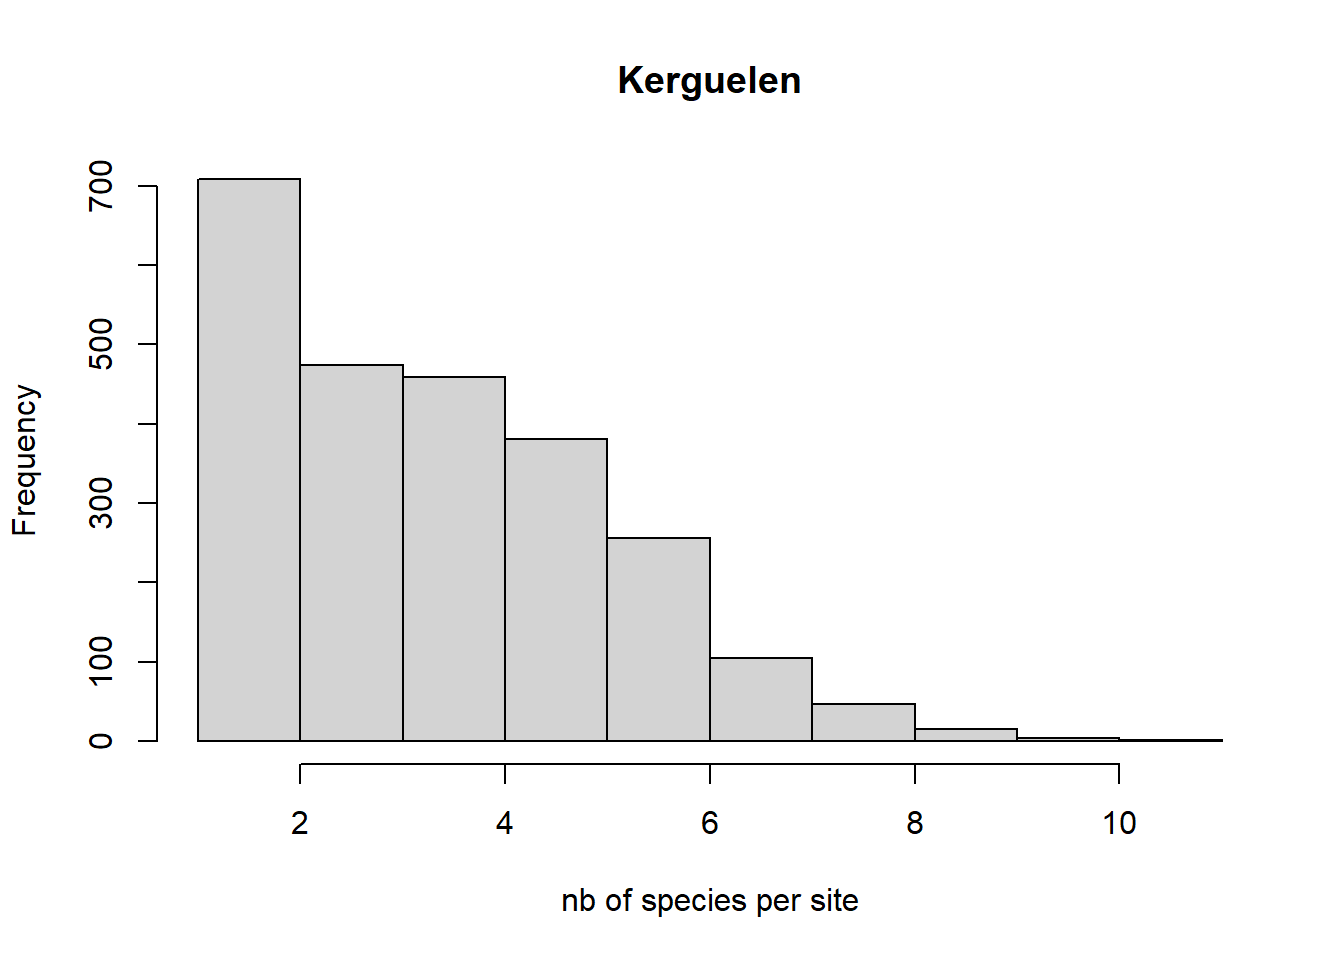
\includegraphics{model_run_files/figure-latex/unnamed-chunk-3-1.pdf}

Still no traits, and there wil be none from TRY ==\textgreater{} not
enough traits measured across all plant species.

HMSC also needs the followong :

\begin{Shaded}
\begin{Highlighting}[]
\CommentTok{\# STUDY DESIGN}
\NormalTok{studyDesign }\OtherTok{=} \FunctionTok{data.frame}\NormalTok{(}\AttributeTok{site=}\NormalTok{XData}\SpecialCharTok{$}\NormalTok{numero\_observation, }\AttributeTok{id=}\NormalTok{XData}\SpecialCharTok{$}\NormalTok{id)}

\CommentTok{\# RANDOM EFFECT STRUCTURE, HERE Site (hierarchical study design)}
\NormalTok{rL.site }\OtherTok{=}\NormalTok{ Hmsc}\SpecialCharTok{::}\FunctionTok{HmscRandomLevel}\NormalTok{(}\AttributeTok{units =} \FunctionTok{levels}\NormalTok{(studyDesign}\SpecialCharTok{$}\NormalTok{site))}
\FunctionTok{str}\NormalTok{(rL.site)}
\end{Highlighting}
\end{Shaded}

\begin{verbatim}
## List of 18
##  $ pi           : Factor w/ 1956 levels "C10A01","C10A02",..: 1 2 3 4 5 6 7 8 9 10 ...
##  $ s            : NULL
##  $ sDim         : num 0
##  $ spatialMethod: NULL
##  $ x            : NULL
##  $ xDim         : num 0
##  $ N            : int 1956
##  $ distMat      : NULL
##  $ nfMax        : num Inf
##  $ nfMin        : num 2
##  $ nNeighbours  : NULL
##  $ nu           : num 3
##  $ a1           : num 50
##  $ b1           : num 1
##  $ a2           : num 50
##  $ b2           : num 1
##  $ alphapw      : NULL
##  $ call         : language Hmsc::HmscRandomLevel(units = levels(studyDesign$site))
##  - attr(*, "class")= chr "HmscRandomLevel"
\end{verbatim}

Not too sure what this does in detail, but it has default parameters to
estimate the random effects. I didn't alter this.

\begin{Shaded}
\begin{Highlighting}[]
\CommentTok{\# and optionally id, if we are interested in species associations at that level}
\NormalTok{rL.id }\OtherTok{=}\NormalTok{ Hmsc}\SpecialCharTok{::}\FunctionTok{HmscRandomLevel}\NormalTok{(}\AttributeTok{units =} \FunctionTok{levels}\NormalTok{(studyDesign}\SpecialCharTok{$}\NormalTok{id))}
\FunctionTok{str}\NormalTok{(rL.site)}
\end{Highlighting}
\end{Shaded}

\begin{verbatim}
## List of 18
##  $ pi           : Factor w/ 1956 levels "C10A01","C10A02",..: 1 2 3 4 5 6 7 8 9 10 ...
##  $ s            : NULL
##  $ sDim         : num 0
##  $ spatialMethod: NULL
##  $ x            : NULL
##  $ xDim         : num 0
##  $ N            : int 1956
##  $ distMat      : NULL
##  $ nfMax        : num Inf
##  $ nfMin        : num 2
##  $ nNeighbours  : NULL
##  $ nu           : num 3
##  $ a1           : num 50
##  $ b1           : num 1
##  $ a2           : num 50
##  $ b2           : num 1
##  $ alphapw      : NULL
##  $ call         : language Hmsc::HmscRandomLevel(units = levels(studyDesign$site))
##  - attr(*, "class")= chr "HmscRandomLevel"
\end{verbatim}

Same structure as the site random level, except this one is supposed to
be much finer, at the observation scale.

\hypertarget{model-structure}{%
\subsection{Model structure}\label{model-structure}}

\begin{Shaded}
\begin{Highlighting}[]
\CommentTok{\# REGRESSION MODEL FOR ENVIRONMENTAL COVARIATES.}
\NormalTok{XFormula }\OtherTok{=} \ErrorTok{\textasciitilde{}}\NormalTok{ mean\_temp }\SpecialCharTok{+}\NormalTok{ accum\_prec }\SpecialCharTok{+}\NormalTok{ pente }\SpecialCharTok{+}\NormalTok{ exposition}

\CommentTok{\# REGRESSION MODEL FOR TRAITS : none.}

\CommentTok{\# PRESENCE{-}ABSENCE MODEL FOR INDIVIDUAL SPECIES (COMMON ONLY)}
\NormalTok{m }\OtherTok{=}\NormalTok{ Hmsc}\SpecialCharTok{::}\FunctionTok{Hmsc}\NormalTok{(}\AttributeTok{Y=}\NormalTok{Y, }\AttributeTok{XData =}\NormalTok{ XData,  }\AttributeTok{XFormula =}\NormalTok{ XFormula,}
         \CommentTok{\# TrData = TrData, TrFormula = TrFormula,}
         \AttributeTok{phyloTree =}\NormalTok{ phylo\_cro,}
         \AttributeTok{distr=}\StringTok{"probit"}\NormalTok{,}
         \AttributeTok{studyDesign =}\NormalTok{ studyDesign, }\AttributeTok{ranLevels=}\FunctionTok{list}\NormalTok{(}\AttributeTok{site=}\NormalTok{rL.site, }\AttributeTok{id=}\NormalTok{rL.id))}
\end{Highlighting}
\end{Shaded}

\hypertarget{model-fit}{%
\subsection{Model fit}\label{model-fit}}

input parameters :

\begin{itemize}
\item
  nChains = 4
\item
  nParallel = nChains
\item
  samples=250, thin=1000
\end{itemize}

\begin{Shaded}
\begin{Highlighting}[]
\NormalTok{m }\OtherTok{=}\NormalTok{ Hmsc}\SpecialCharTok{::}\FunctionTok{sampleMcmc}\NormalTok{(m, }\AttributeTok{samples =}\NormalTok{ samples, }\AttributeTok{thin=}\NormalTok{thin,}
               \AttributeTok{adaptNf=}\FunctionTok{rep}\NormalTok{(}\FunctionTok{ceiling}\NormalTok{(}\FloatTok{0.4}\SpecialCharTok{*}\NormalTok{samples}\SpecialCharTok{*}\NormalTok{thin),m}\SpecialCharTok{$}\NormalTok{nr), }
               \AttributeTok{transient =} \FunctionTok{ceiling}\NormalTok{(}\FloatTok{0.5}\SpecialCharTok{*}\NormalTok{samples}\SpecialCharTok{*}\NormalTok{thin),}
               \AttributeTok{nChains =}\NormalTok{ nChains,}
               \AttributeTok{nParallel =}\NormalTok{ nParallel) }
\end{Highlighting}
\end{Shaded}

\hypertarget{results}{%
\subsection{Results}\label{results}}

See pdf called ``results/parameter\_estimates\_ex2.pdf'').

\begin{itemize}
\tightlist
\item
  Variance partitioning plot: The corresponding values are in
  ``results/parameter\_estimates\_VP\_presence\_absence\_model.csv''
\end{itemize}

There's also this : ``results/parameter\_estimates\_VP\_R2T\_Beta.csv''
: it looks at the beta estimates for each level of the environmental
factor variables, but it didn't work (NAs). Not sure why but doesn't
matter too much for us I think.

\begin{itemize}
\item
  Beta plot : the posterior beta estimates for each plant * covariate.
  Corresponding values in ``results/parameter\_estimates\_Beta\_
  presence-absence model.xls''
\item
  Omega plots : associations between species at the site and id level.
\end{itemize}

\hypertarget{evaluate-model-fit}{%
\subsection{Evaluate model fit}\label{evaluate-model-fit}}

I'm not sure I did this right.

nfolds = NULL \#Default: two-fold cross-validation. There's a place in
the code where I think we're supposed to specify the column (variable)
over which the fold should be done. I didn't..

It's all stored in the
``models/MF\_thin\_1000\_samples\_250\_chains\_4\_nfolds\_2.RData'', and
the results are in ``results/model\_fit\_nfolds\_2.pdf''. But I don't
understand these plots.

\hypertarget{make-predictitons}{%
\subsection{Make predictitons}\label{make-predictitons}}

See the ``results/predictions.pdf''.

\end{document}
